\subsection{Serviço de Proxy -- Squid}

O serviço de proxy tem a função de encaminhar os pedidos para a
Internet e guardar uma \emph{cache} dos conteúdos de forma a acelerar a
visualização dos mesmos quando forem novamente consultados pelos
utilizadores.

O ficheiro que define o modo de funcionamento do proxy é o /etc/squid/squid.conf
que está dividido nas seguintes áreas:

\begin{itemize}
\item Configurações globais: contém definições globais de
funcionamento

\item Autenticação: define os programas de autenticação (para o browser)

\item ACLs: define que tipos de condicionantes são passíveis de utilizar

\item External ACLs: define condicionantes utilizando programas externos
ao proxy

\item Parents: indicação de quais os proxies em cadeia a utilizar e quais
os condicionantes

\item Acessos: define as combinações de acls de modo a filtrar o tráfego
\end{itemize}

\subsubsection{Configurações globais}

A secção de configurações globais permite mudar
parametrizações de funcionamento do servidor nomeadamente onde
são guardados os logs do proxy, o utilizador com o qual o proxy vai a
ser executado, a porta onde está à espera dos pedidos dos
utilizadores, etc.

De seguida são apresentadas algumas das opções possíveis de
configurar nesta secção bem como uma breve descrição.


\confoption{http\_port}

\begin{description}
\item[Utilização]~\\
\texttt{http\_port \emph{port}\\
hostname: port\\
1.2.3.4 : port}

\item[Descrição]~\\
Esta directiva é usada para especificar o socket onde o proxy vai
escutar os pedidos dos browsers. Vários sockets podem ser
especificados.

Existem três formas de utilizar esta directiva: porta apenas, nome
da máquina e porta, e endereço IP e porta.
Se for definido o nome da máquina ou o endereço IP, o proxy vai
apenas escutar nesse interface de rede.

\item[Default]~\\
\texttt{http\_port 3128}

\item[Exemplo]~\\
\texttt{http\_port 8080}

Deste modo vai escutar na porta 8080 reescrevendo a configuração
por omissão.
\end{description}

\confoption{visible\_hostname}

\begin{description}
\item[Utilização]~\\
\texttt{visible\_hostname \emph{anyhostname}}

\item[Descrição]~\\
Define o nome da máquina visível nas mensagens de erro.

\item[Default]~\\
--

\item[Exemplo]~\\
\texttt{visible\_hostname proxy.eurotux.com}
\end{description}

\confoption{cache\_effective\_user}

\begin{description}
\item[Utilização]~\\
\texttt{cache\_effective\_user \emph{userid}}

\item[Descrição]~\\
Se o proxy é executado como root vai mudar o seu userid para o
especificado.

O valor usado por omissão é nobody.

\item[Default]~\\
\texttt{cache\_effective\_user nobody}

\item[Exemplo]~\\
\texttt{cache\_effective\_user squid}
\end{description}


\confoption{error\_directory}

\begin{description}
\item[Utilização]~\\
\texttt{error\_directory \emph{directorypath/directoryname}}

\item[Descrição]~\\
Define a localização das mensagens de erro.

\item[Default]~\\
Normalmente em \emph{/etc/squid/errors}.

\item[Exemplo]~\\
\texttt{error\_directory /etc/errors}
\end{description}

\confoption{icon\_directory}

\begin{description}
\item[Utilização]~\\
\texttt{icon\_directory \emph{directorypath/directoryname}}

\item[Descrição]~\\
Esta opção define onde os icons estão guardados.

\item[Default]~\\
Normalmente em \emph{/etc/squid/icons}.

\item[Exemplo]~\\
\texttt{icon\_directory /etc/icons}
\end{description}

\subsubsection{Autenticação}

A secção de Autenticação define quais os programas de
autenticação, ou seja, os programas que perguntam ao
browser/utilizador qual os seus dados de autenticação.
Estão definidos dois modelos de autenticação: \emph{basic}
(quando o browser não suporta autenticação transparente
aparece um popup para introdução de dados) ou \emph{ntlmssp}
(autenticação transparente do utilizador).

\confoption{auth\_param}

\begin{description}
\item[Utilização]~\\
\texttt{auth\_param \emph{type} \emph{params} \emph{[options]}}

Descrição dos parâmetros suportados (\emph{params}):

\begin{description}
\item[program]~\\
Especifica o programa utilizado para autenticação.  
Tal programa irá ler uma linha contendo ``utilizador password''
e responder ao squid com um ``OK'' para sucesso ou um ``ERR''
para falha.

Para utilizar um autenticador, é necessário uma acl do
tipo proxy\_auth.  
Por norma utiliza-se o sistema de autenticação básico.

\texttt{auth\_param basic program \emph{/path/do/programa}
\emph{/path/do/arquivo/senhas}}

\item[children]~\\
Número de processos filhos que o programa de autenticação
poderá conter

\texttt{auth\_param basic children \emph{número}}

\item[realm]~\\
Texto que irá aparecer na caixa de diálogo de login. Não é
necessário configurar, mas confere uma certa personalização ao
servidor.

\texttt{auth\_param basic realm \emph{Texto de login}}

\item[credentials\_ttl]~\\
Especifica por quanto tempo o Squid irá assumir que uma
autenticação bem sucedida continuará válida.

\texttt{auth\_param basic credentialsttl \emph{tempo}}
\end{description}

\item[Default]~\\
--

\item[Exemplo]~\\
\begin{Output}
auth_param ntlm program /usr/bin/ntlm_auth --helper-protocol=squid-2.5-ntlmssp
auth_param ntlm children 5
auth_param ntlm max_challenge_reuses 0
auth_param ntlm max_challenge_lifetime 20 minutes
auth_param basic program /usr/bin/ntlm_auth --helper-protocol=squid-2.5-basic
auth_param basic children 5
auth_param basic realm Squid proxy-caching web server
auth_param basic credentialsttl 2 hours
\end{Output}
\end{description}

\subsubsection{ACLs}

A secção de ACLs permite definir quais os modelos de filtragem
passíveis de serem utilizados posteriormente na secção de
acessos.

\confoption{acl}

\begin{description}
\item[Utilização]~\\
acl \emph{aclname} \emph{acltype} \emph{string1} ... \textbar{} \emph{file}

\item[Descrição]~\\
Esta tag é utilizada para definir uma lista de acessos.
Quando ``file'' é usado deve conter um item por linha.
Normalmente, as expressões são case-sensitive, para as tornar
case-insensitive, use a opção \emph{-i}.

A acltype pode ser:

\begin{itemize}
\item src
\begin{description}
\item[Descrição] Vai verificar o endereço ip de origem.

\item[Utilização] \texttt{acl \emph{aclname} src
\emph{ip-address/netmask}}

\item[Exemplo]~\\
\texttt{acl aclname src 172.16.1.0/24} -- Refere a rede 172.16.1.0

\texttt{acl aclname src 172.16.1.25/32} -- Refere apenas um endereço de
origem
\end{description}

\item dst
\begin{description}
\item[Descrição] Tem a mesma funcionalidade que o src mas
refere o endereço ip destino.

\item[Utilização] \texttt{acl \emph{aclname} dst
\emph{ip-address/netmask}}

\item[Exemplo]~\\
\texttt{acl localhost src 127.0.0.0/255.255.255.0}
\end{description}
\end{itemize}
\end{description}

\subsubsection{External ACLs}

ACLs externas permitem expandir as funcionalidades do proxy utilizando
para isso programas externos ao mesmo para gerir acessos.
Este tipo de acls permite então, por exemplo, perguntar a um servidor
Active Directory se um determinado utilizador pertence a um grupo, se
um determinado endereço de origem pode fazer pedidos para a internet
com base numa base de dados SQL, etc.

A especificação deste comando é a seguinte:

\confoption{external\_acl\_type}

\begin{description}
\item[Utilização]~\\
\texttt{external\_acl\_type \emph{aclname} \emph{field}
\emph{command}}

\item[Descrição]~\\
Esta tag permite definir uma acl que será validada utilizando o
programa definido e passando no input o campo definido.

\item[Default]~\\
--

\item[Exemplo]~\\
\texttt{external\_acl\_type checkuser \%LOGIN /etc/squid/check\_group.pl
squidguard}

\texttt{external\_acl\_type checkwhite \%LOGIN /etc/squid/check\_group.pl
white}
\end{description}

A criação de uma acl externa pressupõe posteriormente a
criação de uma acl interna com a referência ao nome da acl
externa.
A título de exemplo, a seguinte acl externa:

\texttt{external\_acl\_type checkwhite \%LOGIN /etc/squid/check\_group.pl
white}

pressupõe a existência posterior da seguinte acl:

\texttt{acl whiteuser external checkwhite}

Neste momento usar-se-ia a acl whiteuser.

\subsubsection{Parents}

Esta secção especifica quais os proxies em cadeia que serão
utilizados pelo proxy de entrada para download de informação.

\confoption{cache\_peer}

\begin{description}
\item[Utilização]~\\
\texttt{cache\_peer \emph{hostname} \emph{type}
\emph{http\_port} \emph{icp\_port} \emph{options}}

\item[Descrição]~\\
Esta tag é usada para especificar outros proxies na hierarquia e
está dividida em cinco campos.
O primeiro campo é no nome ou IP do proxy que vai ser utilizado.
O segundo indica o tipo de relação com o proxy seguinte.
O terceiro campo indica a porta HTTP onde o proxy destino vai
escutar os pedidos, e o quarto a porta de ICP.
O quinto campo pode existir ou não e especifica as opções.

\begin{description}
\item[hostname]~\\
Hostname (FQDN) ou endereço IP da cache a ser utilizada.

Por exemplo,

\texttt{cache\_peer a.eurotux.com sibling 3128 3130 [proxy{}-only]}

\texttt{cache\_peer 172.16.1.100 sibling 3128 3130 [proxy{}-only]}

\item[type]~\\
Tipo de hierarquia a utilizar entre os proxies.

\begin{itemize}
\item
\href{http://squid.visolve.com/squid/squid24s1/glossary.htm#parent}{parent}

\item
\href{http://squid.visolve.com/squid/squid24s1/glossary.htm#sibling}{sibling}

\item
\href{http://squid.visolve.com/squid/squid24s1/glossary.htm#multicast}{multicast}
\end{itemize}

\item[http\_port]~\\
A porta onde o proxy seguinte está à espera dos pedidos.

\item[icp\_port]~\\
Usada para perguntar aos vizinhos sobre os objectos que as caches possam
ter ou não.

\item[option]~\\
\begin{description}
\item[\href{http://squid.visolve.com/squid/squid24s1/glossary.htm\#proxy-only}{proxy-only}]~\\
Indica que o conteúdo pedido a este proxy não é para guardar localmente.

\item[\href{http://squid.visolve.com/squid/squid24s1/glossary.htm\#weight}{Weight=n}]~\\
Especifica o peso na escolha do proxy.
Por omissão é 1 e quanto maior for, mais ``favorecido'' será este proxy.

\item[\href{http://squid.visolve.com/squid/squid24s1/glossary.htm\#ttl}{ttl=n}]~\\
Especifica o Time To Live (ttl). Apenas utilizado em multicast.

\item[\href{http://squid.visolve.com/squid/squid24s1/glossary.htm\#no-query}{no-query}]~\\
Usado para proxies que não usam ICP, ou seja, que não indicam se
contêm um objecto ou não.

\item[\href{http://squid.visolve.com/squid/squid24s1/glossary.htm\#default}{default}]~\\
Quando o proxy é o último na linha hierárquica usa-se esta
opção.

\item[\href{http://squid.visolve.com/squid/squid24s1/glossary.htm\#round-robin}{round-robin}]~\\
Para usar proxies em modo round-robin.
\end{description}
\end{description}

\item[Default]~\\
--

\item[Exemplo]~\\
\texttt{cache\_peer proxy.visolve.com parent 3128 3130 default}

\texttt{cache\_peer 172.16.1.100 sibling 3128 3130 proxy-only}

\texttt{cache\_peer 172.16.1.123 sibling 3129 5500 weight=2}
\end{description}

\confoption{cache\_peer\_access}

\begin{description}
\item[Utilização]~\\
\texttt{cache\_peer\_access cache-host allow\textbar{}deny [!]aclname ...}

\item[Descrição]~\\
Usa acls para escolher qual o proxy parent a usar.

\item[Default]~\\
--

\item[Example]~\\
O seguinte exemplo envia todos os pedidos vindos da rede 10.0.1.0 pelo
proxy.

\begin{Output}
acl myNet src 10.0.0.0/255.255.255.0
acl cusNet src 10.0.1.0/255.255.255.0
acl all src 0.0.0.0/0.0.0.0
cache_peer a.eurotux.com parent 3128 3130
cache_peer_access a.eurotux.com allow custNet
cache_peer_access a.eurotux.com deny all
\end{Output}
\end{description}

\subsubsection{Acessos}

Esta secção especifica quais as combinações das acls a
aplicar a cada situação e qual a acção a fazer: negar ou
aceitar.
É de salientar que estas regras são interpretadas de cima
para baixo e caso uma regra seja correspondida a acção é
efectuada.
É importante salientar que caso não exista no final a
opção http\_access deny todos os pedidos que chegarem a esse
ponto são aceites.
A título de exemplo, este funcionamento é o inverso das acls
da Cisco onde a acção por omissão é negar.

\confoption{http\_access}

\begin{description}
\item[Utilização]~\\
\texttt{http\_access allow\textbar{}deny [!]aclname ...}

\item[Descrição]~\\
Permitir ou negar o acesso http baseado em acls.

\item[Default]~\\
\begin{Output}
http_access allow manager localhost
http_access deny manager
http_access deny !Safe_ports
http_access deny CONNECT !SSL_ports
http_access deny all
\end{Output}
\end{description}

\confoption{cache\_dir}

\begin{description}
\item[Utilização]~\\
\texttt{cache\_dir \emph{Type} \emph{Directory-Name} \emph{Mbytes}
\emph{Level-1} \emph{Level2} [..]}

\texttt{DISKD :}

\texttt{cache\_dir diskd \emph{Directory-Name} \emph{MB} \emph{L1}
\emph{L2} \emph{Q1} \emph{Q2}}

\item[Descrição]~\\
O campo \emph{Type} especifica que tipo de sistema de armazenamento vai
utilizar.

\emph{Directory} especifica a directoria onde o proxy vai armazenar os dados.
A directoria tem de existir e tem de ter permissões de escrita para o
utilizador com o qual o proxy está a ser executado.

\emph{Mbytes} é o espaço em MB alocado para armazenamento.

\emph{Level-1} é o número de directorias de primeiro nível criadas
dentro da directoria principal de armazenamento.

\emph{Level-2} especifica o número de directorias de segundo nível a
serem criadas dentro das de primeiro nível.

\item[Default]~\\
\texttt{cache\_dir ufs /usr/local/squid/cache 100 16 256}

\item[Exemplo]~\\
\texttt{cache\_dir ufs /cache1 5000 16 256}

\texttt{cache\_dir ufs /cache2 7000 16 256}
\end{description}

\subsubsection{Exemplos de configurações}

O seguinte capítulo vai incluir alguns exemplos de
configurações.

\paragraph{Restringir acessos por tempo}

Podem ser criadas ACLs baseadas em parâmetros temporais.
Aqui ficam alguns exemplos.
É necessário reniciar o squid para as alterações ficarem
activas

Aceitar acessos da rede interna em horas de trabalho:

\begin{Output}
# Adicionar o seguinte no final da secção das acls
acl home_network src 192.168.1.0/24
acl business_hours time M T W H F 9:00-17:00

# Adicionar o seguinte no início da secção de http_access
http\_access allow home_network business_hours
\end{Output}

Aceitar acessos apenas de manhã:

\begin{Output}
# Adicionar o seguinte no final da zona de acls
acl mornings time 08:00-12:00

# Adicionar o seguinte no início da zona de http_access
http\_access allow mornings
\end{Output}

\paragraph{Restringir acessos pelo endereço IP}

Podemos restringir os acessos à internet baseado nos endereços de
origem.
Neste caso estamos a criar uma ACL que define a nossa rede como
192.168.1.0.

\begin{Output}
# Adicionar no final da zona de acls
acl home_network src 192.168.1.0/255.255.255.0
\end{Output}

É também necessário adicionar o correspondente http\_access para
permitir tráfego que corresponde à ACL.

\begin{Output}
# Adicionar no início da zona de http_access
http_access allow home_network
\end{Output}

\paragraph{Proxy Transparente}

Um proxy transparente permite ter um sistema de cache totalmente
invisível dos browsers.
Para tal é necessária a colaboração do router de saída que
encaminhe todos os pedidos web vindos da rede interna para o proxy.
É importante salientar que não é possível criar um proxy
transparente para o protocolo https, pelas garantias de
confidencialidade que são inerentes ao próprio protocolo, bem como
não é possível ter autenticação de utilizadores.

A configuração do proxy é então a seguinte a acrescentar na
zona de configuração global:

\begin{Output}
httpd_accel_host virtual
httpd_accel_port 80
httpd_accel_with_proxy on
httpd_accel_uses_host_header on
\end{Output}

É ainda necessário reencaminhar no router todos os pedidos web para
o ip do proxy na porta 80.

\subsubsection{Operações sobre o serviço}

As operações sobre este serviço são:

\ServiceCommands{squid}

\subsubsection{Exemplos de utilização}

Nesta sub-secção vamos abordar alguns exemplos de configurações mais comuns de modo a que possa facilmente efectuar qualquer alteração no seu serviço.
Embora tenhamos anteriormente especificadas as opções que o servidor permite, necessitaria de aceder ao servidor via SSH, alterar o ficheiro de configuração do squid (/etc/squid/squid.conf) e reiniciar o serviço para que as alterações fossem activadas. Embora este acesso seja o preferêncial para utilizadores com conhecimentos de Linux, é disponibilizado um acesso web de administração para gerir o seu proxy.

No primeiro exemplo vamos abordar a negação do acesso a determinadas páginas com URLs baseados em padrões.

\subsubsection{Negar acesso baseado em RegEXP no URL}

Para negar o acesso a determinados endereços web (URLs) baseado num qualquer texto que faça parte do mesmo devemos aceder à interface web de administração do seu proxy (tipicamente em http://XXX.XXX.XXX.XXX:12345/ ou http://XXX.XXX.XXX.XXX:10000/ onde XXX.XXX.XXX.XXX é o endereço ip do seu servidor de proxy). Depois de inserir as credenciais deverá escolher na árvore do lado esquerdo, na secção "Servers", o item "Squid Proxy Server".

Deverá ver algo como a seguinte imagem:

\begin{figure}[H]
    \begin{center}
        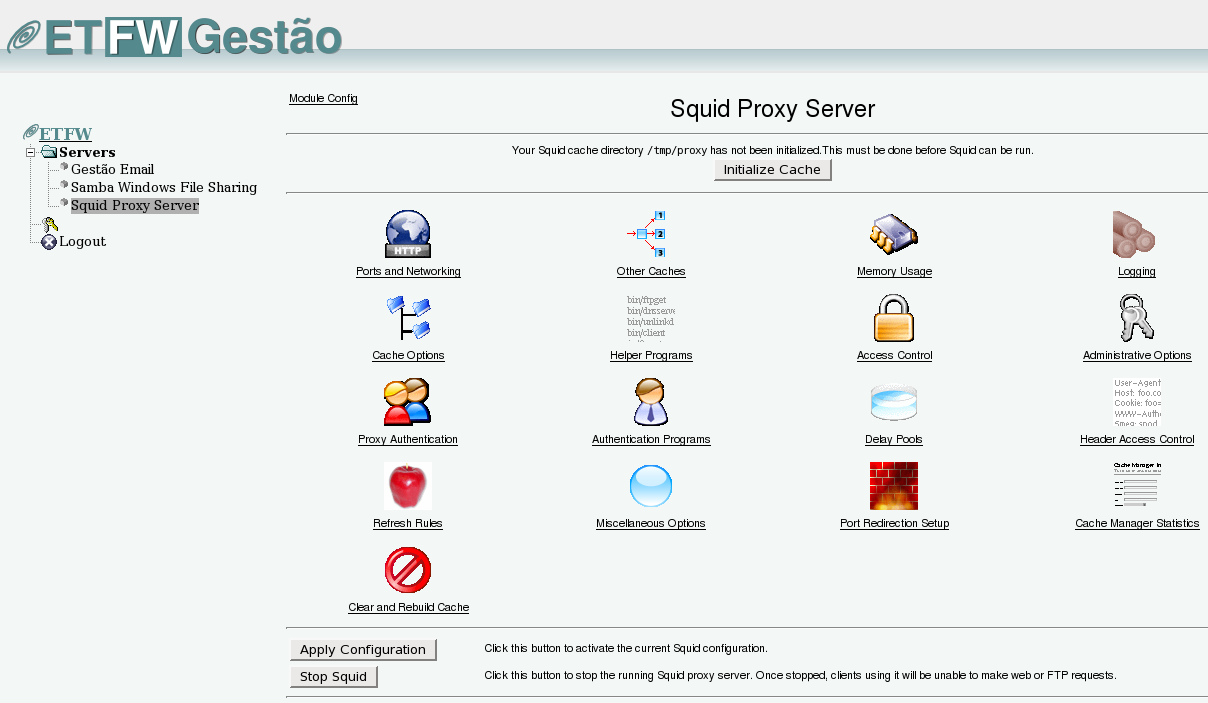
\includegraphics[width=10cm]{include/img/squid1}
    \end{center}
    \caption{Administração do Proxy}
    \label{fig:SQUID1}
\end{figure}

Deverá posteriormente escolher a opção "Access Control" e deverá ver algo como a seguinte imagem:

\begin{figure}[H]
    \begin{center}
        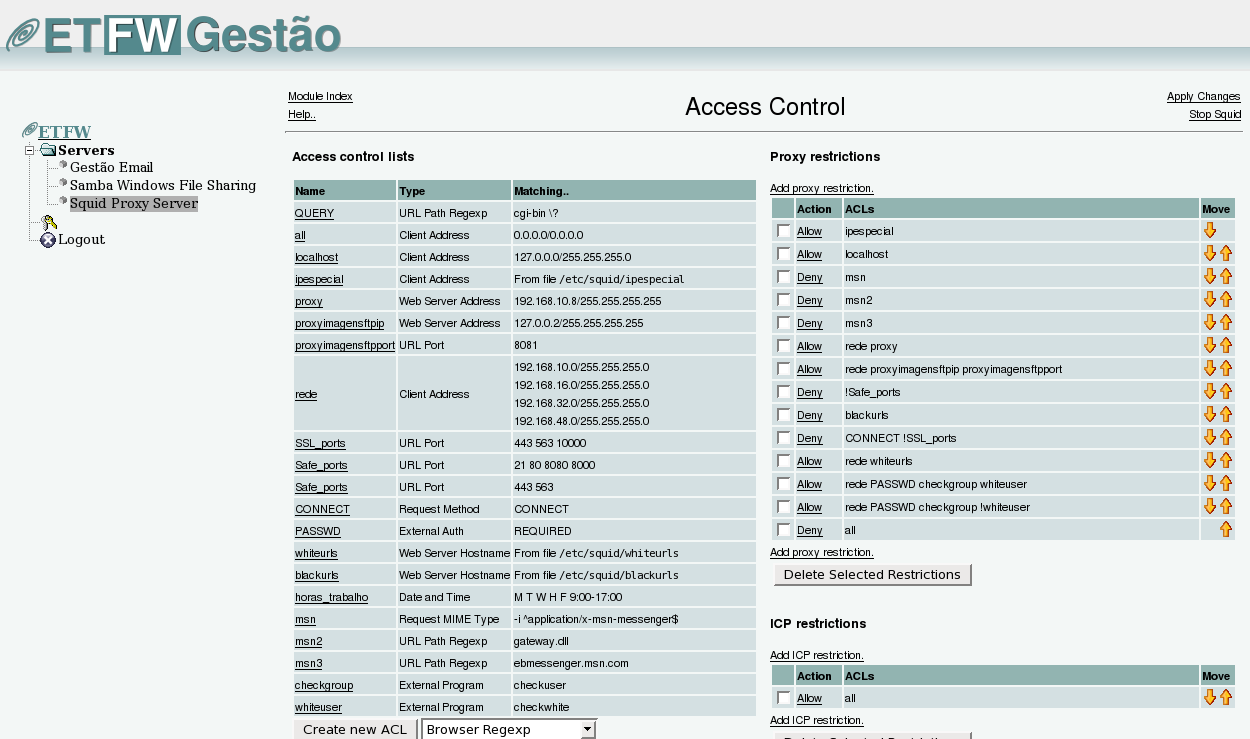
\includegraphics[width=10cm]{include/img/squid2}
    \end{center}
    \caption{Acl do Proxy}
    \label{fig:SQUID2}
\end{figure}

De seguida deverá escolher a opção "URL Regexp" e carregar no botão "Create New ACL".

\begin{figure}[H]
    \begin{center}
        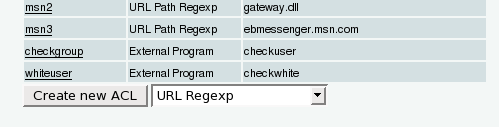
\includegraphics[width=10cm]{include/img/squid3}
    \end{center}
    \caption{Acls do Proxy}
    \label{fig:SQUID3}
\end{figure}

Deverá de seguida ser apresentada uma página como a seguinte:

\begin{figure}[H]
    \begin{center}
        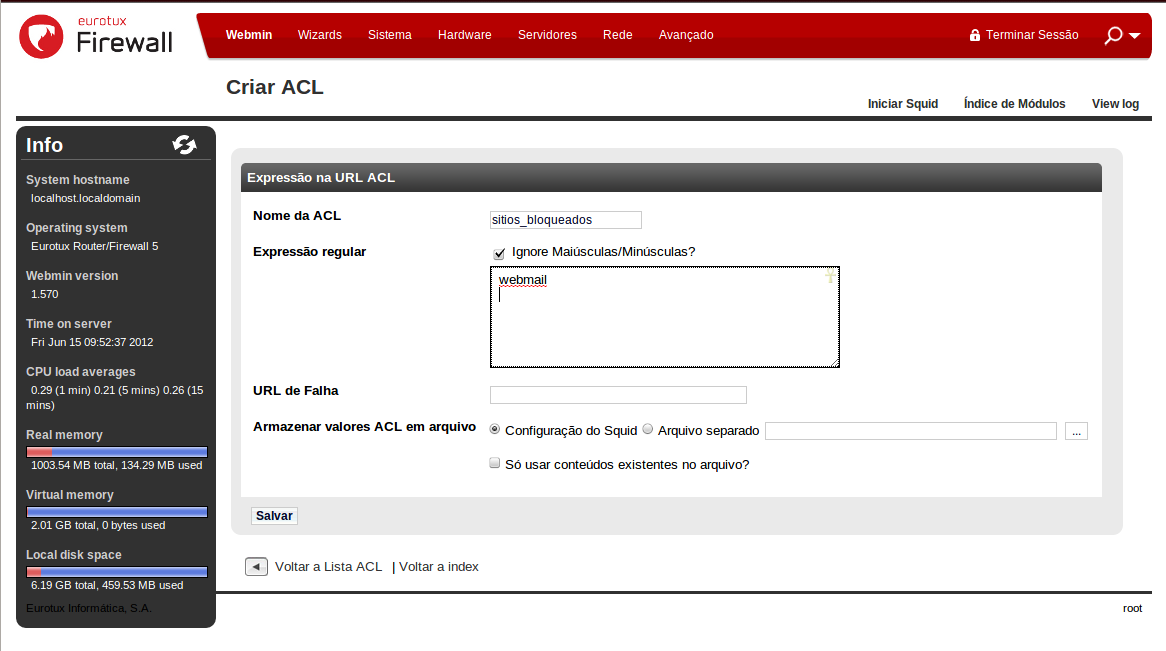
\includegraphics[width=10cm]{include/img/squid4}
    \end{center}
    \caption{Criar URL Regexp}
    \label{fig:SQUID4}
\end{figure}

Após carregar em "Save" voltará à página inicial das ACLs. Vamos agora aplicar este filtro para negar o acesso a estes sites. Para tal deverá escolher o link "Add proxy restriction" que é apresentado abaixo de "Proxy restrictions".

\begin{figure}[H]
    \begin{center}
        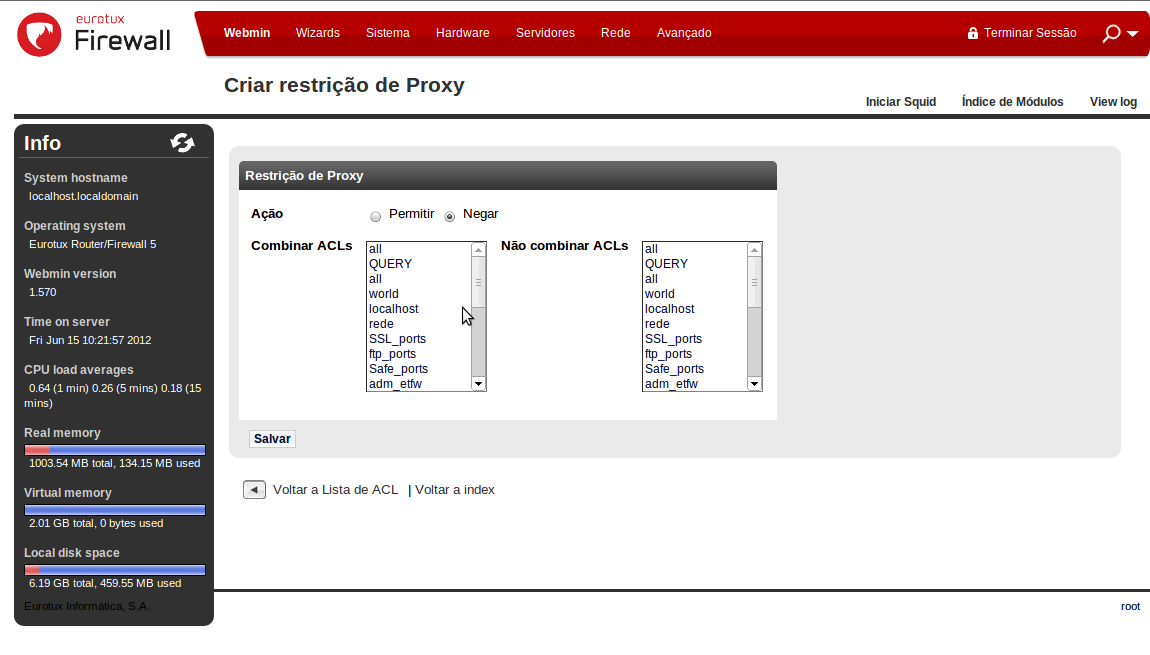
\includegraphics[width=10cm]{include/img/squid5}
    \end{center}
    \caption{Adicionar uma restrição de proxy}
    \label{fig:SQUID5}
\end{figure}

Vamos então escolher a acção que será despoletada quando alguém aceder a estes sites. Neste caso vamos escolher a acção "Deny" e vamos de seguida definir o padrão que criámos anteriormente (sitios\_bloqueados).

\begin{figure}[H]
    \begin{center}
        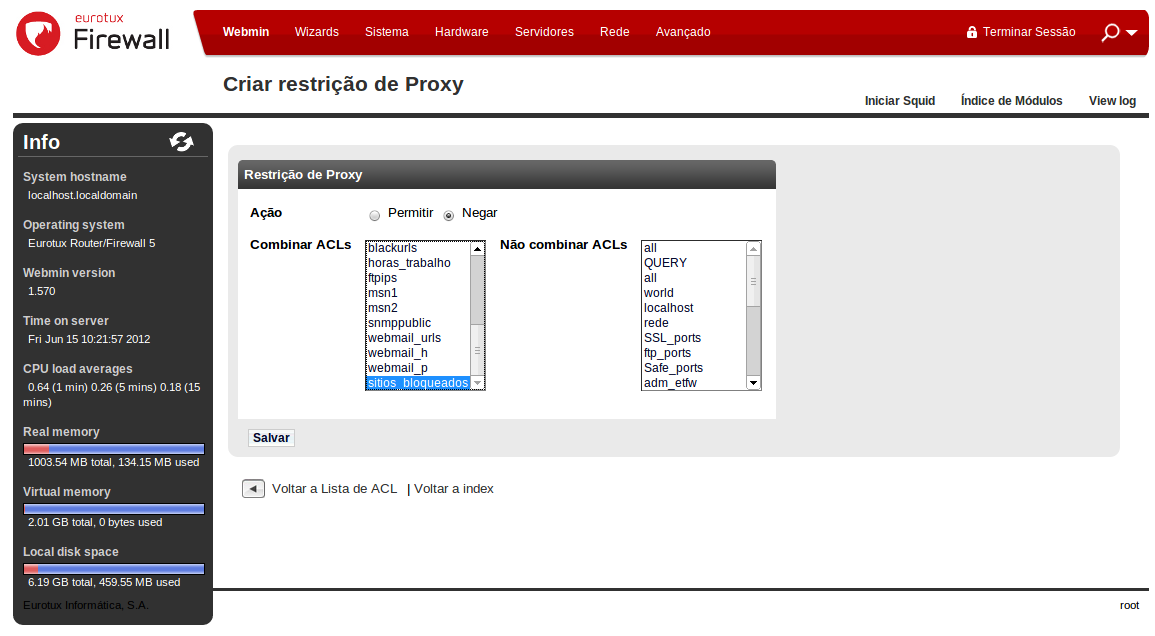
\includegraphics[width=10cm]{include/img/squid6}
    \end{center}
    \caption{Adicionar uma restrição de proxy - Guardar}
    \label{fig:SQUID6}
\end{figure}


Após gravarmos a alteração, voltaremos à interface de acls onde podemos encontrar a nova acl.

\begin{figure}[H]
    \begin{center}
        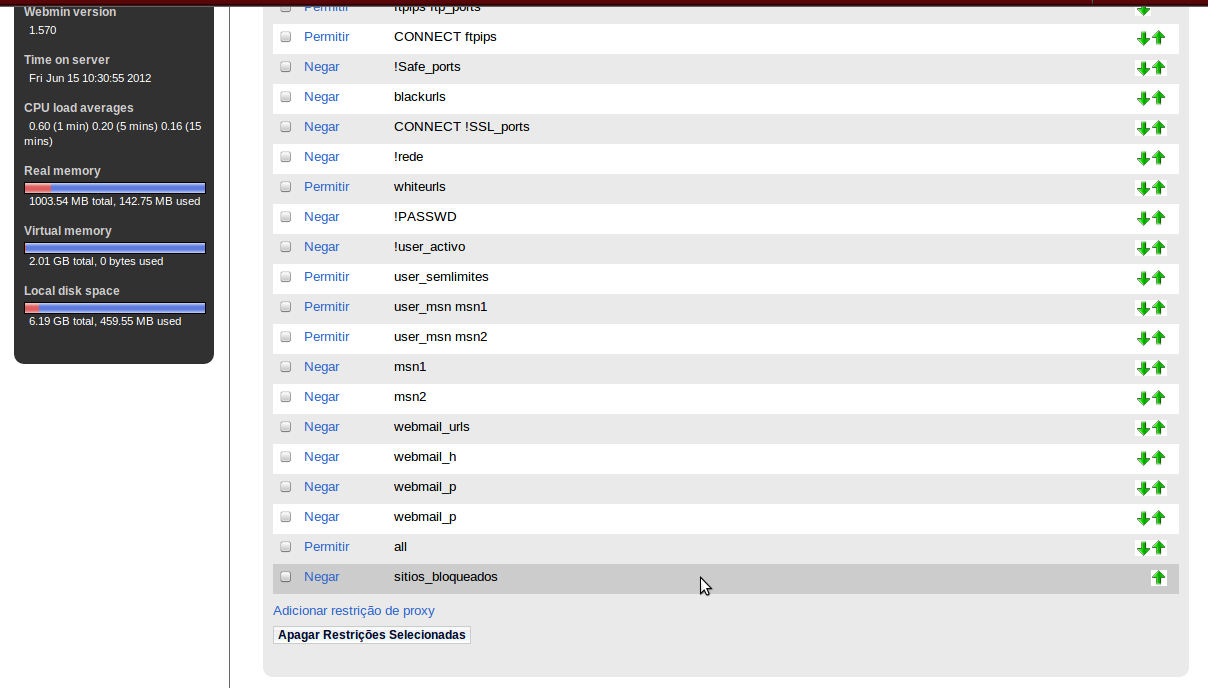
\includegraphics[width=10cm]{include/img/squid7}
    \end{center}
    \caption{Adicionar uma restrição de proxy - Menu}
    \label{fig:SQUID7}
\end{figure}


Devemos de seguida colocar a acl acima na cadeia de verificações carregando na seta amarela para cima. Deverá ficar antes da directiva "Allow 	rede PASSWD checkgroup whiteuser".

Após esta modificação deverá aplicar as alterações carregando no link "Apply Changes" que se encontra no canto superior direito.
